\documentclass[border=2pt]{standalone}
\usepackage{tikz}
\begin{document}
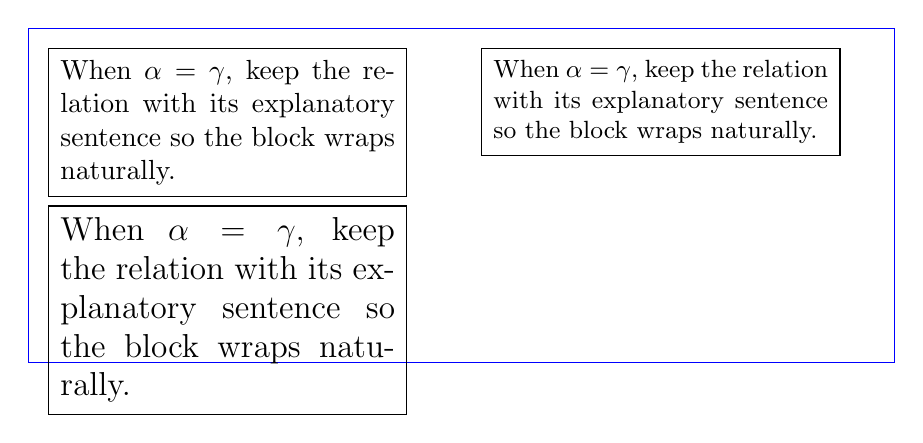
\begin{tikzpicture}
  \draw[blue] (-.25,-4) rectangle (10.75,.25);
  \node[draw,anchor=north west,inner sep=1ex] at (0,0) {
    \begin{minipage}{4.25cm}
      When $\alpha = \gamma$, keep the relation with its explanatory sentence
      so the block wraps naturally.
    \end{minipage}
  };
  \node[draw,anchor=north west,inner sep=1ex,font=\small] at (5.5,0) {
    \begin{minipage}{4.25cm}
      When $\alpha = \gamma$, keep the relation with its explanatory sentence
      so the block wraps naturally.
    \end{minipage}
  };
  \node[draw,anchor=north west,inner sep=1ex,font=\large] at (0,-2) {
    \begin{minipage}{4.25cm}
      When $\alpha = \gamma$, keep the relation with its explanatory sentence
      so the block wraps naturally.
    \end{minipage}
  };
\end{tikzpicture}
\end{document}
